\begin{SCn}

\scnsectionheader{\currentname}

\scnstartsubstruct

\scnheader{Предметная область структур}
\scnsdmainclasssingle{структура}
\scnsdclass{связная структура;несвязная структура;тривиальная структура;нетривиальная структура;структура второго уровня;семантический уровень структурного элемента;количество семантических уровней элементов структуры}

\scnsdrelation{элемент структуры’;непредставленное множество’;полностью представленное множество’;частично представленное множество’;элемент структуры, не являющийся множеством';максимальное множество’;немаксимальное множество’;первичный элемент’;вторичный элемент’;элемент второго уровня’;метасвязь’;полиморфность*;полиморфизм*;гомоморфность*;гомоморфизм*;изоморфность*;изоморфизм*;автоморфность*;автоморфизм*;аналогичность структур*;сходство*;различие*;первичная синтаксическая структура sc-текста*}

\scnheader{структура}
\scnidtf{sc-структура}
\scnidtf{структура, представленная в виде текста SC-кода}
\scnreltoset{разбиение}{связная структура;несвязная структура}
\scnreltoset{разбиение}{тривиальная структура;нетривиальная структура}
\scnexplanation{\textbf{\textit{структура}} — множество \textit{sc-элементов}, удаление одного из которых может привести к нарушению целостности этого множества.}

\scnheader{связная структура}
\scnexplanation{\textit{Структуре}, представленной в \textit{SC-коде}, поставим в соответствие орграф, вершинами которого являются \textit{sc-элементы}, а дугами – пары инцидентности, связывающие \textit{sc-коннекторы} с инцидентными им \textit{sc-элементами}, которые являются компонентами указанных \textit{sc-коннекторов}.

Если полученный таким способом орграф является связным орграфом, то исходную структуру будем считать \textbf{\textit{связной структурой}}.}

\scnheader{несвязная структура}
\scnexplanation{\textit{Структуре}, представленной в \textit{SC-коде}, поставим в соответствие орграф, вершинами которого являются \textit{sc-элементы}, а дугами – пары инцидентности, связывающие \textit{sc-коннекторы} с инцидентными им \textit{sc-элементами}, которые являются компонентами указанных \textit{sc-коннекторов}.

Если полученный таким способом орграф не является связным орграфом, то исходную структуру будем считать \textbf{\textit{несвязной структурой}}.}

\scnheader{тривиальная структура}
\scnidtf{структура первого уровня}
\scnexplanation{\textbf{\textit{тривиальная структура}} – \textit{структура}, не содержащая в качестве элементов связок.}

\scnheader{нетривиальная структура}
\scnsuperset{структура второго уровня}
\scnexplanation{\textbf{\textit{нетривиальная структура}} – \textit{структура}, среди элементов которой есть хотя бы одна связка.}

\scnheader{элемент структуры’}
\scniselement{неосновное понятие}
\scnreltoset{разбиение}{непредставленное множество';полностью представленное множество’;частично представленное множество’;элемент структуры, не являющийся множеством'}
\scnreltoset{разбиение}{максимальное множество’;немаксимальное множество'}
\scnexplanation{\textbf{\textit{элемент структуры'}} — \textit{неосновное понятие}, \textit{ролевое отношение}, указывающее на все элементы каждой структуры.

В рамках заданной структуры ее элементы можно классифицировать по заданным признакам:
\begin{scnitemize}
\item насколько полно в рамках \underline{заданной \textit{структуры}} представлено множество, обозначаемое \textit{заданным sc-элементом} вместе с соответствующими дугами принадлежности;
\item существуют ли в рамках \underline{заданной \textit{структуры}} \textit{sc-элементы}, обозначающие множества, являющиеся надмножествами того множества, которое обозначается \underline{заданным \textit{sc-элементом}};
\item уровень («этаж») иерархии перехода от знаков к метазнакам для \underline{заданного \textit{sc-элемента}} в рамках заданной \textit{структуры}.
\end{scnitemize}
}

\scnheader{непредставленное множество’}
\scnidtf{множество, не представленное в рамках данной структуры’}
\scnidtf{быть знаком множества, элементы которого не являются элементами данной структуры'}
\scniselement{ролевое отношение}
\scnexplanation{\textbf{\textit{непредставленное множество’}} – \textit{ролевое отношение}, связывающее структуру со знаком множества, все элементы которого не являются элементами данной структуры.}

\scnheader{полностью представленное множество’}
\scnidtf{множество, полностью представленное в рамках данной структуры'}
\scnidtf{множество, все элементы которого являются элементами данной структуры'}
\scnidtf{полностью представленный класс'}
\scniselement{ролевое отношение}
\scnexplanation{\textbf{\textit{полностью представленное множество’}} – \textit{ролевое отношение}, связывающее \textit{структуру} со знаком множества (любого семантического типа – класса, связки или структуры), все элементы которого являются элементами данной \textit{структуры}.}

\scnheader{частично представленное множество’}
\scnidtf{множество, частично представленное в рамках данной структуры'}
\scnidtf{множество, некоторые элементы которого являются элементами данной структуры'}
\scnidtf{быть знаком множества, некоторые элементы которого являются элементами данной структуры'}
\scniselement{ролевое отношение}
\scnexplanation{\textbf{\textit{частично представленное множество’}} – ролевое отношение, связывающее структуру со знаком множества, не все элементы которого являются элементами данной структуры.}

\scnheader{элемент структуры, не являющийся множеством’}
\scniselement{ролевое отношение}

\scnheader{максимальное множество’}
\scnexplanation{\textbf{\textit{максимальное множество’}} – \textit{ролевое отношение}, связывающее \textit{структуру} со знаком множества, для которого не существует множества, которое было бы надмножеством указанного множества и знак которого был бы элементом этой же структуры.}

\scnheader{немаксимальное множество’}
\scnexplanation{\textbf{\textit{немаксимальное множество’}} – \textit{ролевое отношение}, связывающее \textit{структуру} со знаком множества, для которого в рамках данной \textit{структуры} существует множество, являющееся надмножеством указанного множества.}

\scnheader{первичный элемент’}
\scnidtf{первичный элемент данной структуры'}
\scnidtf{sc-элемент первого уровня в рамках данной структуры'}
\scniselement{ролевое отношение}
\scniselement{семантический уровень структурного элемента}
\scnsubset{элемент структуры’}
\scnexplanation{\textbf{\textit{первичный элемент’}} – ролевое отношение, указывающее на элемент \textit{структуры}, являющийся либо терминальным элементом, либо знаком множества, такого что не существует другого элемента этой же структуры, который был бы элементом множества, обозначаемого первым из указанных элементов структуры. При этом соответствующая пара принадлежности может существовать, но в состав данной структуры не входить.}

\scnheader{вторичный элемент’}
\scnidtf{вторичный элемент данной структуры’}
\scnidtf{элемент данной структуры имеющий семантический уровень более 2'}
\scnidtf{непервичный элемент'}
\scniselement{ролевое отношение}
\scnsubset{элемент структуры’}
\scnexplanation{\textbf{\textit{вторичный элемент’}} – ролевое отношение, указывающее на элемент структуры, обозначающий множество, все или некоторые элементы которого являются элементами указанной структуры.}
\scnsuperset{элемент второго уровня’}

\scnheader{элемент второго уровня’}
\scniselement{ролевое отношение}
\scniselement{семантический уровень структурного элемента}
\scnexplanation{\textbf{\textit{элементом второго уровня’}} в рамках заданной \textit{структуры} может быть связка первичных элементов, тривиальная структура из первичных элементов или класс первичных элементов.}

\scnheader{структура второго уровня’}
\scnexplanation{\textbf{\textit{структура второго уровня}} - \textit{структура}, среди элементов которой есть хотя бы один \textit{элемент второго уровня’}.}

\scnheader{семантический уровень структурного элемента}
\scniselement{параметр}
\scnexplanation{\textbf{\textit{семантический уровень структурного элемента}} представляет собой \textit{параметр}, каждый элемент которого является классом 
\textit{sc-дуг принадлежности}, связывающих некоторую \textit{структуру} с теми ее элементами, который имеют одинаковый семантический уровень в рамках данной структуры. Значением данного параметра является число, обозначающее указанный семантический уровень.

\textbf{\textit{семантический уровень структурного элемента}} вычисляется следующим образом:

\begin{scnitemize}
\item элементы структуры, входящие в нее с атрибутом \textit{первичный элемент'} имеют семантический уровень 1;
\item уровень элемента, не являющегося \textit{первичным элементом'} структуры вычисляется путем прибавления 1 к максимальному из уровней элементов этого элемента (множества), входящих в эту же структуру. Например, \textit{sc-дуга}, соединяющая два \textit{первичных элемента' структуры} будет иметь семантический уровень 2, а \textit{sc-элемент}, обозначающий отношение, которому принадлежит указанная \textit{sc-дуга} – семантический уровень 3.
\end{scnitemize}
}
\scnrelfrom{типичная семантическая окрестность}{
\scnfilelong{
\begin{figure}[H]
\centering
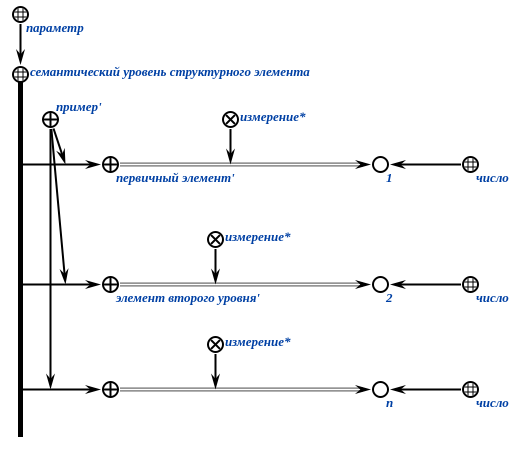
\includegraphics[width=0.7\linewidth]{figures/sd_structures/sem_level_struct_elem.png}
\end{figure}
}}

\scnheader{количество семантических уровней элементов структуры}
\scniselement{параметр}
\scnexplanation{\textbf{\textit{количество семантических уровней элементов структуры}} – параметр, каждый элемент которого представляет собой класс структур, у которых совпадает максимальный среди семантических уровней элементов этих структур.


Значением данного параметра является число, совпадающее с указанным максимальным семантическим уровнем элементов.}

\scnheader{метасвязь’}
\scniselement{ролевое отношение}
\scnsubset{вторичный элемент’}
\scnexplanation{
\begin{scnenumerate}
    \item Каждая входящая в структуру связь, хотя бы одним компонентом которой является связь, входящая в эту же структуру, элементами которой являются \textit{первичные элементы’} этой структуры, является \textbf{\textit{метасвязью’}} указанной структуры;
    \item Каждая входящая в структуру связь, хотя бы одним компонентом которой является \textbf{\textit{метасвязь’}} этой структуры также является \textbf{\textit{метасвязью’}} указанной структуры;
\end{scnenumerate}
}

\scnheader{полиморфность*}
\scnsubset{соответствие*}
\scniselement{бинарное отношение}
\scnexplanation{\textbf{\textit{полиморфность*}} - это \textit{соответствие}, заданное на \textit{структурах}, при котором каждому элементу из области определения соответствия (первой \textit{структуры}) ставится в соответствие один или более элемент из области значения соответствия (второй \textit{структуры}), при этом существует хотя бы один элемент области определения соответствия, которому соответствуют два или более элемента из области значения соответствия.}

\scnheader{полиморфизм*}
\scniselement{бинарное отношение}

\scnheader{гомоморфность*}
\scnidtf{гомоморфность структур*}
\scnsubset{соответствие*}
\scniselement{бинарное отношение}
\scnexplanation{\textbf{\textit{гомоморфность*}} - это \textit{соответствие}, заданное на \textit{структурах}, при котором каждому элементу из области определения соответствия (первой \textit{структуры}) ставится в соответствие только один элемент из области значения соответствия (второй \textit{структуры}).}
\scnrelfrom{типичная семантическая окрестность}{
\scnfilelong{
\begin{figure}[H]
\centering
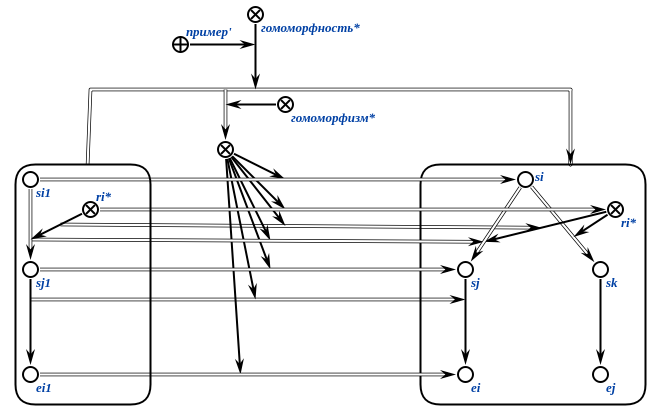
\includegraphics[width=1\linewidth]{figures/sd_structures/homomorphism.png}
\end{figure}
}}

\scnheader{гомоморфизм*}
\scniselement{бинарное отношение}

\scnheader{изоморфность*}
\scnidtf{изоморфное соответствие*}
\scnidtf{изоморфность структур*}
\scnsubset{гомоморфность*}
\scniselement{бинарное отношение}
\scnexplanation{\textbf{\textit{изоморфность*}} - это \textit{гомоморфность*}, при которой для каждого элемента из области значения существует ровно один соответствующий элемент из области определения.}
\scnrelfrom{типичная семантическая окрестность}{
\scnfilelong{
\begin{figure}[H]
\centering
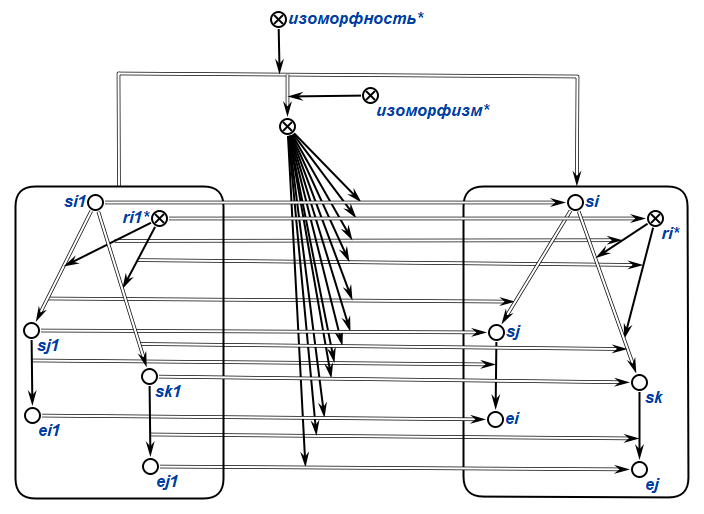
\includegraphics[width=1\linewidth]{figures/sd_structures/isomorphism.png}
\end{figure}
}}

\scnheader{изоморфизм*}
\scniselement{бинарное отношение}

\scnheader{автомоморфность*}
\scnsubset{гомоморфность*}
\scniselement{бинарное отношение}
\scnexplanation{\textbf{\textit{автоморфность*}} - это \textit{изоморфность*}, у которой область определения соответствия и область значения соответствия совпадают.}
\scnrelfrom{типичная семантическая окрестность}{
\scnfilelong{
\begin{figure}[H]
\centering
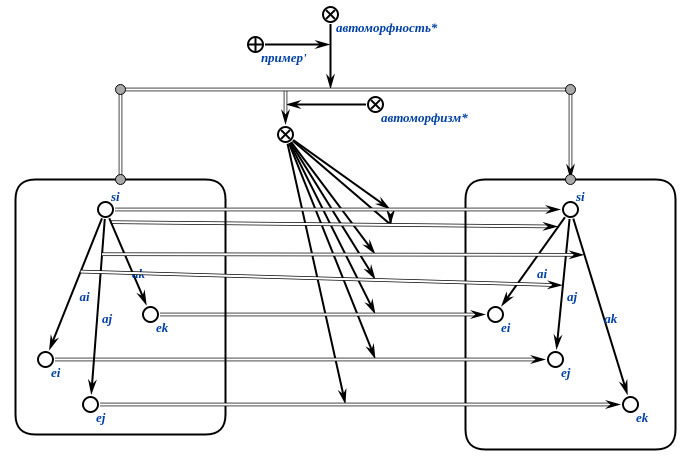
\includegraphics[width=1\linewidth]{figures/sd_structures/automorphism.png}
\end{figure}
}}

\scnheader{автоморфизм*}
\scniselement{бинарное отношение}

\scnheader{аналогичность структур*}
\scnsubset{соответствие*}
\scniselement{бинарное отношение}
\scnexplanation{\textbf{\textit{аналогичность структур*}} - \textit{соответствие*}, задаваемое на структурах, и фиксирующее факт наличия некоторой аналогии на подструктурах (подмножествах) указанных структур. Каждой ориентированной паре, принадлежащей \textbf{\textit{аналогичности структур*}} может быть поставлено в соответствие множество пар, задающих \textit{сходства*} некоторых подструктур и \textit{различия*} некоторых подструктур исходных структур.}
\scnrelfrom{типичная семантическая окрестность}{
\scnfilelong{
\begin{figure}[H]
\centering
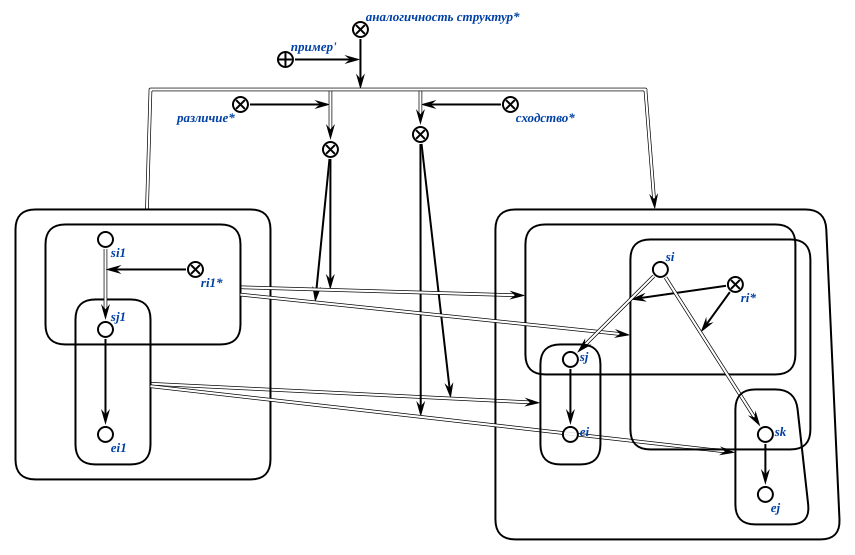
\includegraphics[width=1\linewidth]{figures/sd_structures/analogy.png}
\end{figure}
}}

\scnheader{сходство*}
\scniselement{бинарное отношение}

\scnheader{различие*}
\scniselement{бинарное отношение}

\scnheader{первичная синтаксическая структура sc-текста*}
\scniselement{бинарное отношение}
\scnexplanation{\textbf{\textit{первичная синтаксическая структура sc-текста*}} - это бинарное отношение, связывающее некоторый \textit{sc-текст} с другим \textit{sc-текстом}, формируемым по следующим правилам:
\begin{scnitemize}
    \item каждому \textit{sc-узлу} первого \textit{sc-текста} соответствует \textit{синглетон} (\textit{знак sc-узла}) в рамках второго \textit{sc-текста};
    \item каждому \textit{sc-коннектору} из первого \textit{sc-текста} в рамках второго \textit{sc-текста} соответствует \textit{синглетон}, обозначающий данный \textit{sc-коннектор} и соединенный с другими \textit{синглетонами} второго \textit{sc-текста} парами инцидентности двух типов, в зависимости от того, началом или концом данного \textit{sc-коннектора} являются обозначаемые этими \textit{синглетонами sc-элементы}. В случае, когда \textit{sc-коннектор} является \textit{sc-ребром}, то достаточно пар инцидентности первого типа.
    \item для каждого \textit{синглетона} в рамках второго \textit{sc-текста} явно указывается синтаксический тип, определяемый типом соответствующего ему элемента из первого \textit{sc-текста} (\textit{знак sc-константы}, \textit{знак sc-узла} и т.п.).
\end{scnitemize}


Стоит отметить, что подобным образом может быть задана синтаксическая структура любого текста, а не только sc-текста. В этом случае понадобятся другие отношения инцидентности другие классы синтаксических типов.}
\scnrelfrom{типичная семантическая окрестность}{
\scnfilelong{
\begin{figure}[H]
  \centering
  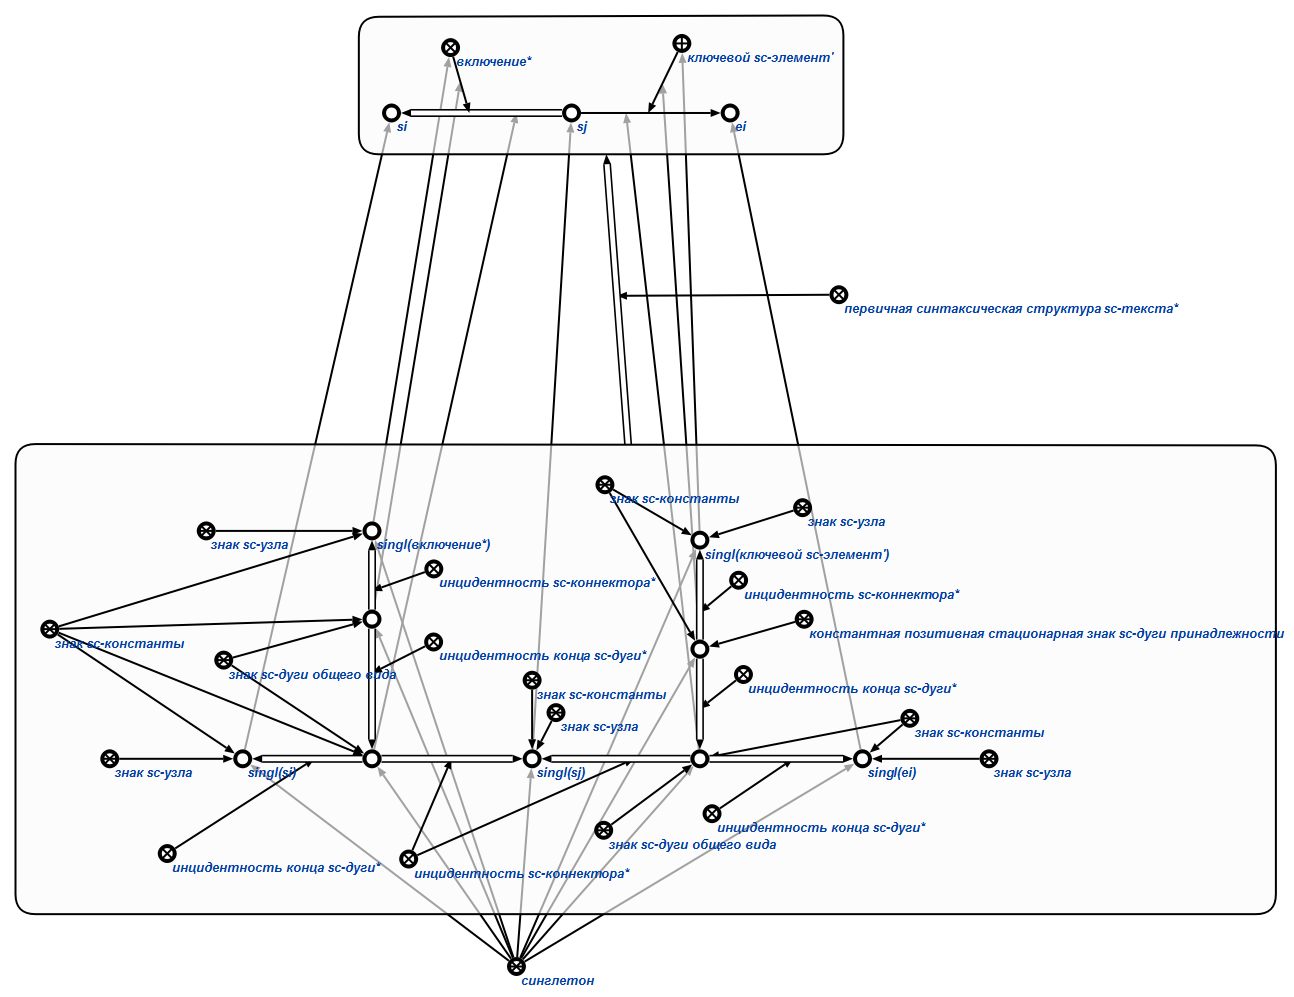
\includegraphics[width=1\linewidth]{figures/sd_structures/primary_sc_syntax.png}
\end{figure}
}}

\scnendstruct

\end{SCn}